\chapter{ЭКСПЕРИМЕНТАЛЬНЫЕ РЕЗУЛЬТАТЫ}

\section{Подготовка данных}

Для проведения экспериментов были получены данные видеосъёмки дроном Phantom DJI 4. Из этих видеороликов мной были подготовлены \textit{наборы данных} (\textbf{data sets}). Экспериментально было установлено, что для того чтобы получить $70\%$ перекрытие на соседних изображениях (необходимое условия для хорошего сопоставления) требуется нарезать видео с частотой хотя бы 1 кадр в 2 секунды. Отдельно рассматривались прямые и обратные (в другую сторону) пролеты БПЛА над одной и той же местностью, для возможности имитации задачи возвращения дрона домой по построенной карте.

\begin{figure}[h]
    \centering
    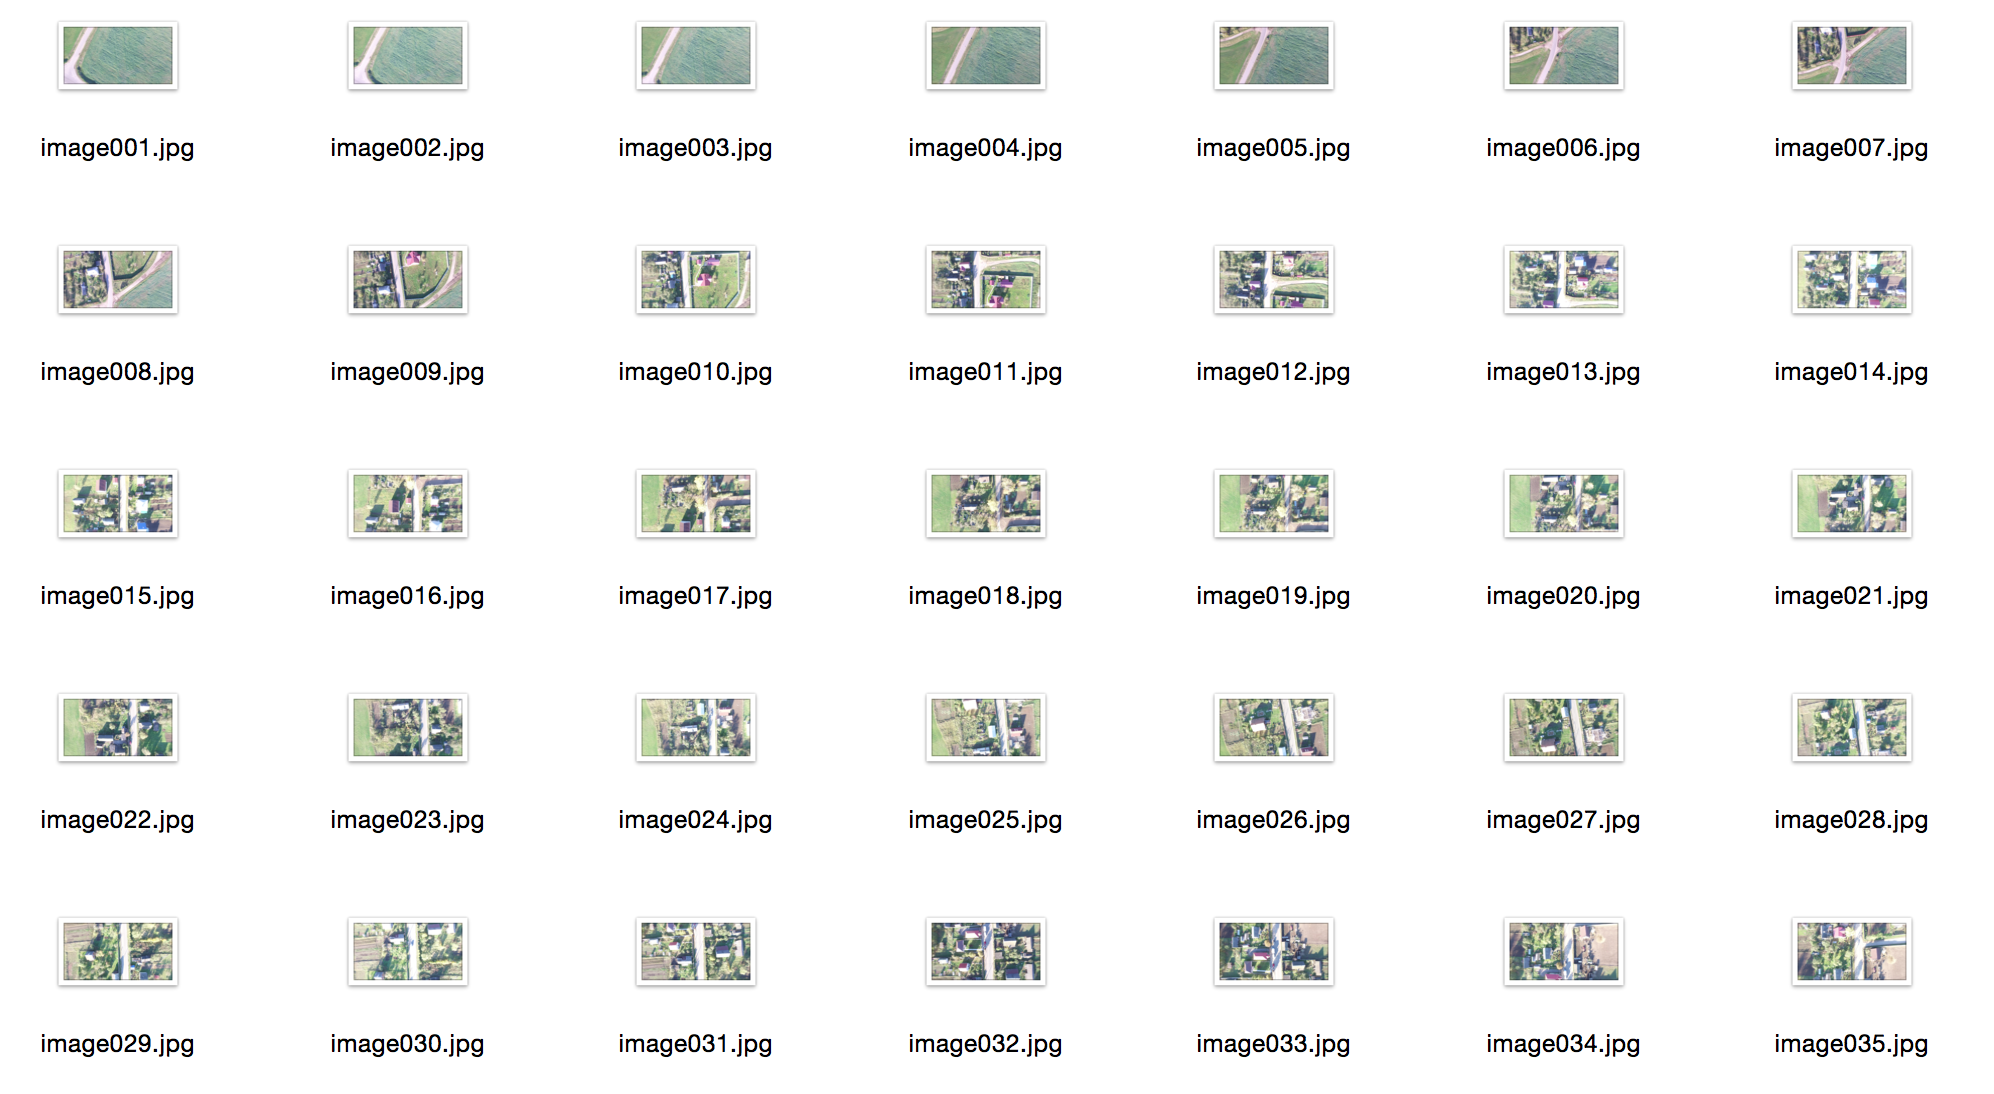
\includegraphics[width=0.8\textwidth]{dataset.png}
    \caption{Снимки полученные с БПЛА}
    \label{fig:dataset}
\end{figure}

\section{Matching эксперименты}

Как первое приближение (начальные данные, от которых впоследствии можно будет отталкиваться) был взят следующий простой алгоритм: каждый снимок сделанный на прямом пролете (кривая $AB$) сопоставляется с каждым снимком из обратного (кривая $BA$). Для $n$ прямых снимков и $m$ обратных получаем $n*m$ сравнений. В итоге для $\forall$ пары снимков $\{i, j | i=\overline{1,n}, j=\overline{1,m}\}$ получаем \textit{результат сравнения} (\textbf{score}) их ключевых точек, на основе которого можно судить соответствуют ли эти снимки одной и той же точке в пространстве.

Мной была написана реализация этого алгоритма на языке программирования $Python$, используя \hyperref[itm:sift]{SIFT [\ref{itm:sift}]} и \hyperref[itm:orb]{ORB [\ref{itm:orb}]} в реализации \hyperref[itm:opencv]{OpenCV [\ref{itm:opencv}]}. В качестве параметров скрипт принимает название алгоритма и максимальное количество ключевых точек, которые будут выделятся на изображении.

\begin{figure}[h]
    \centering
    \includegraphics[width=0.8\textwidth]{features.png}
    \caption{Найденные ключевые точки}
    \label{fig:features}
\end{figure}

\begin{figure}[h]
    \centering
    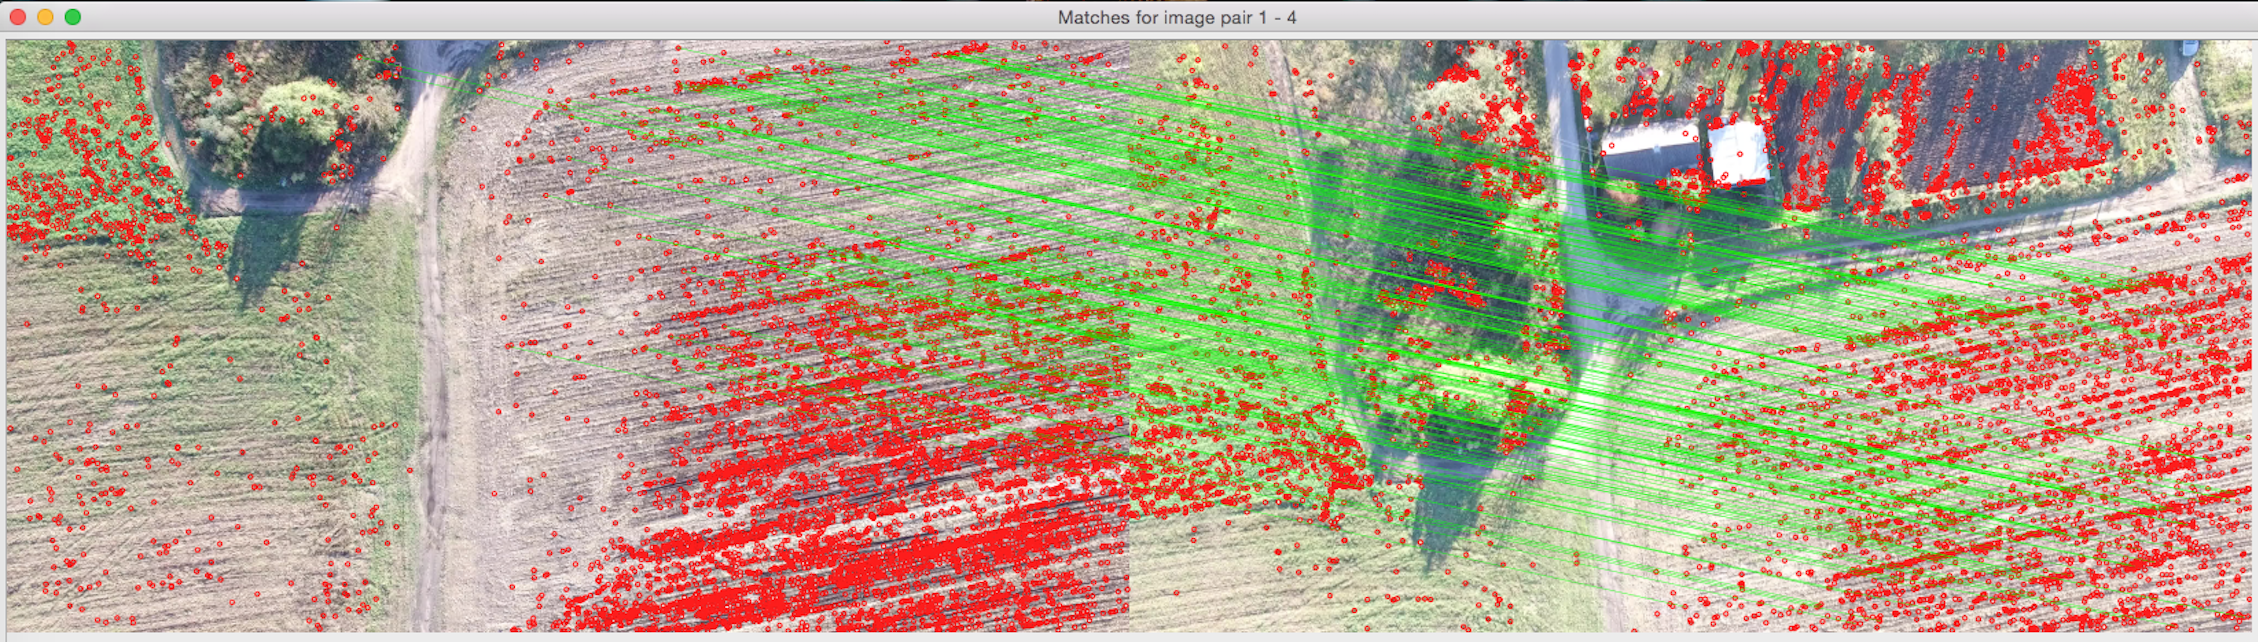
\includegraphics[width=1.0\textwidth]{matches.png}
    \caption{Совпадения ключевых точек}
    \label{fig:matches}
\end{figure}

Варьируя количество выделяемых ключевых точек и используя разные алгоритмы, были поставлены эксперименты. Для визуализации качества сопоставления были построены \textit{тепловые карты} (\textbf{heatmaps}) - диаграммы показывающие насколько хорошо совпадает изображение $x_i$ с $y_j$ (расположены соответственно на осях абсцисс и ординат). Чем выше score сопоставления $x_i$ с $y_j$ изображения, тем \quotes{теплее} этот пиксель на диаграмме.

Сопоставление можно считать успешным, если на диаграмме хорошо прослеживается траектория: так как при пролётах туда-обратно мы должны получать, что на $x_0$ и $y_n$, $x_1$ и $y_{n-1}$ ... и т.д. видны одни и те же точки пространства. Также анализировалось время работы программы. На рисунке \ref{fig:heatmaps} представлены полученные результаты на наборах из 40x32 изображений (1280 сравнений). Легенда изображений: \textit{алгоритм - количество точек - время работы}.

\begin{figure}[h]
    \centering
    \begin{subfigure}[h]{0.45\textwidth}
        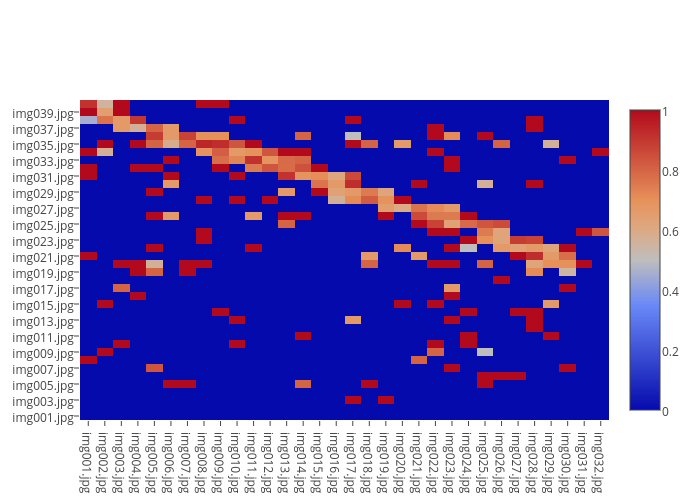
\includegraphics[width=\textwidth]{orb_heatmap200.png}
        \caption{ORB - 200 точек - 18 мин.}
        \label{fig:orb_200}
    \end{subfigure}
    ~ 
    \begin{subfigure}[h]{0.45\textwidth}
        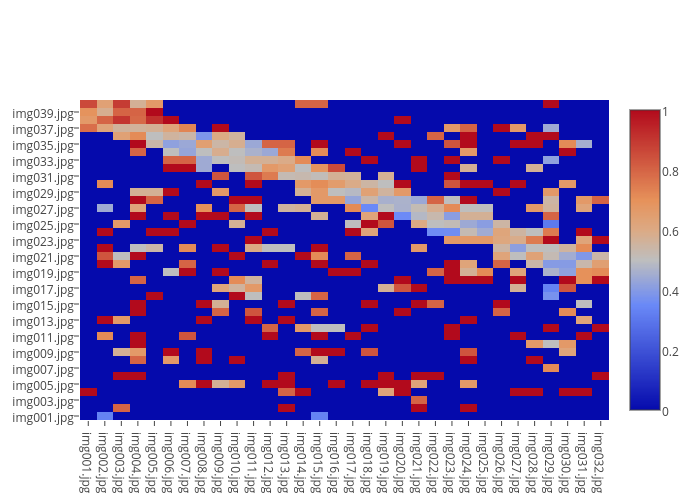
\includegraphics[width=\textwidth]{sift_heatmap200.png}
        \caption{SIFT - 200 точек - 3,7 ч.}
        \label{fig:sift_200}
    \end{subfigure}
    ~ 
    \begin{subfigure}[h]{0.45\textwidth}
        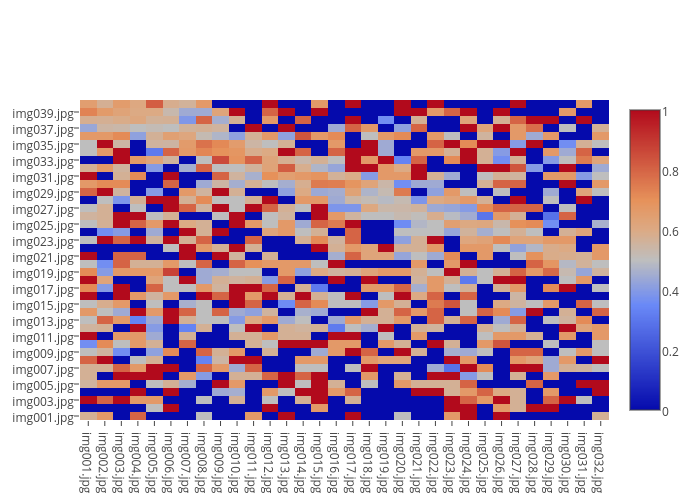
\includegraphics[width=\textwidth]{orb_heatmap1000.png}
        \caption{ORB - 1000 точек - 26 мин.}
        \label{fig:mouse}
    \end{subfigure}
    ~
    \begin{subfigure}[h]{0.45\textwidth}
        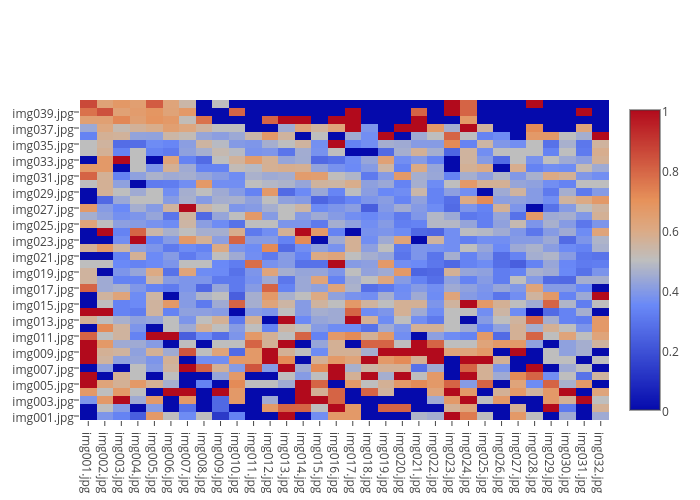
\includegraphics[width=\textwidth]{sift_heatmap1000.png}
        \caption{SIFT - 1000 точек - 4 ч.}
        \label{fig:mouse}
    \end{subfigure}
    \caption{Сравнительные тепловые диаграммы}
    \label{fig:heatmaps}
\end{figure}

\section{Выводы}

Проанализировав диаграммы на рисунке \ref{fig:heatmaps}, можно сделать вывод, что при малом количестве выделяемых ключевых точек прослеживается траектория полёта. Также заметно, что $SIFT$ даёт много ложных сопоставлений при очень большом времени работы - 3,5 часа против 20 минут у $ORB$. Однако при увеличении точек совпадения \quotes{размазываются} по всей диаграмме, это значит, что ошибка растёт и нужно улучшать методы feature extraction для получения лучших ключевых точек.

Учитывая время работы и полученные результаты при большом числе извлекаемых точек, навигация с использованием этого алгоритма, конечно же, не представляется возможной. Однако мы получили первое приближение, решение \quotes{в лоб}, от которого можно отталкиваться в дальнейшем и сравнивать с ним результаты будущей работы.

\newpage